\documentclass{beamer}
\usepackage{Res/tex/presento}

\usepackage{amsfonts, amssymb, amsmath, amsthm, enumerate}
\usepackage{xcolor, graphicx, tikz}
\usepackage{multicol}

\newcommand{\Nat}{\ensuremath \mathbb{N}}
\newcommand{\Int}{\ensuremath \mathbb{Z}}
\newcommand{\Rat}{\ensuremath \mathbb{Q}}
\newcommand{\Real}{\ensuremath \mathbb{R}}
\newtheorem*{teo}{Teorema}
\newtheorem*{df}{Definicija}
\newenvironment{thinker}{\begin{alertblock}{Zavrzlama}}{\end{alertblock}}
\newenvironment{construct}{\begin{block}{Skalamerija}}{\end{block}}
\newenvironment{idea}{\begin{block}{Ideja}}{\end{block}}
\newenvironment{sidenote}{\begin{alertblock}{Inače}}{\end{alertblock}}
\newcommand{\Background}[2]{
    \tikz[remember picture, overlay] \node[opacity=#2, at=(current page.center)] {
        \includegraphics[height=\paperheight]{#1}
    };
}

\begin{document}
    % {
\usebackgroundtemplate{%
\tikz[overlay,remember picture] \node[opacity=0.5, at=(current page.center)] {
  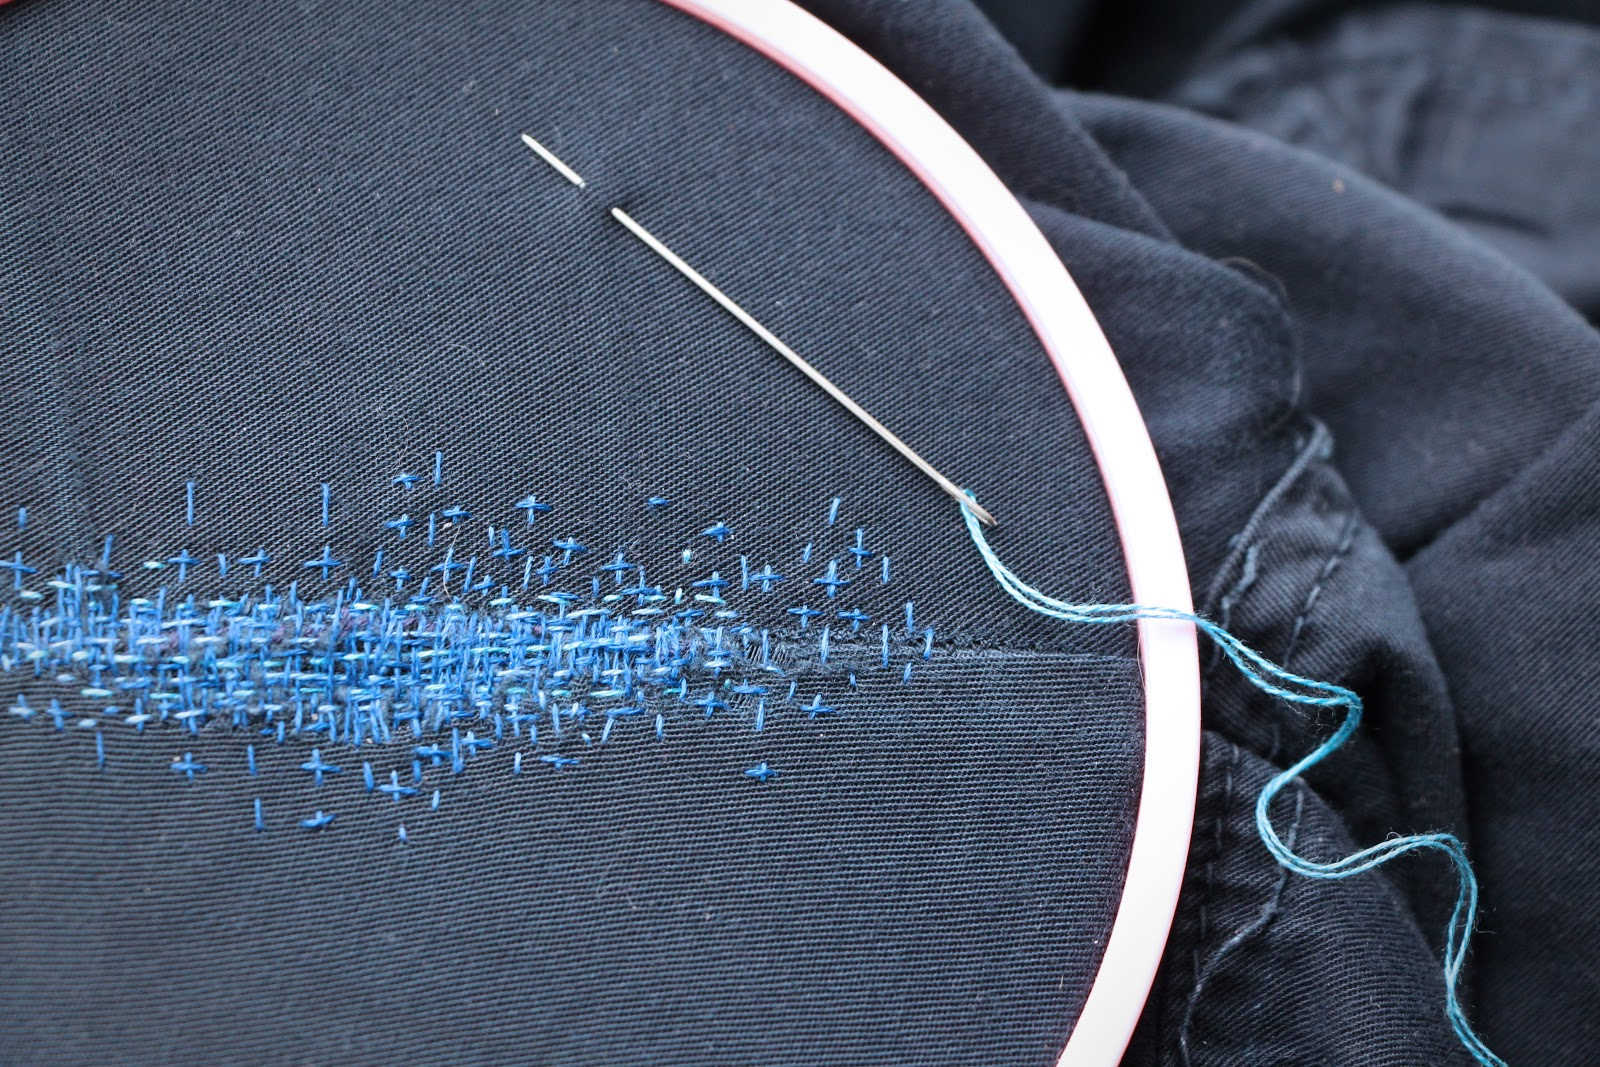
\includegraphics[height=\paperheight]{Res/img/krpljenje}};
}
\begin{frame}[plain]
    \vfill
    \largetext{
        \color{orange}{Dimitrije Glukčević  \\
        \setnote{dimchee90@gmail.com}}
    }
    \scalebox{0.5}{\input{Res/img/pmf.pdf_tex}}
    \vfill
    \largetext{\color{colorblue}
        O raznizavanju i krpljenju
    } \\
    \setnote{Zimski seminar za mlađe polaznike, Petnica 2022}
\end{frame}
}

    % \begin{frame}{Lakiranje rama}
    %     \Background{Res/img/coating}{0.5}
    % \end{frame}
    % \framecard{\Huge{Lakiranje kocke?}}
    % 
    % \begin{frame}{}
    %     \Background{Res/img/operation}{0.5}
    % \end{frame}
    % \begin{frame}{Grupe}
    %     \Background{Res/img/group}{0.5}
    %     \begin{enumerate}
    %         \itemR $(a \circ b) \circ c = a \circ (b \circ c)$
    %         \itemR $\exists e \forall a \quad a \circ e = e \circ a = a$
    %         \itemR $\forall a \exists a^{-1}  \quad a \circ a^{-1} = a^{-1} \circ a = e$
    %         \item[${\color{magenta} \rightarrow}$] $a \oplus b = b \oplus a$
    %     \end{enumerate}
    % \end{frame}
    % \framecard{\Huge{Na koliko načina možemo da rotiramo kocku?}}
    % \begin{frame}{Izomorfizmi}
    %     \Background{Res/img/reflection}{0.7}
    %     \begin{df}[Permutacija]
    %         Permutacija je bilo koja bijekcija skupa u samog sebe.
    %     \end{df}
    %     \begin{teo}[Kejli]
    %         Svaka grupa je izomorfna nekoj grupi permutacija
    %     \end{teo}
    % \end{frame}
    \begin{frame}{Kocka je bačena (jer je loše izlakirana)}
        \Background{Res/img/rubic}{0.5}
        $$S_4 \cong \langle s_1, s_2, s_3 \mid 
            s_1^2 = s_2^2 = s_3^2 = (s_1s_2)^2 = (s_2s_3)^3 = (s_1s_3)^3 = e \rangle
        $$
        \begin{idea}
            Svaki dan farbamo 3, a ne 1 stranu!
        \end{idea}
    \end{frame}
    \begin{frame}{Geometrijska začkoljica}
        \Background{Res/img/geometry}{0.7}
        \begin{thinker}
            Kako predstaviti kretanje po prostoru?
        \end{thinker}
        %\pause
        \begin{thinker}
            Šta su vektori?
        \end{thinker}
    \end{frame}
    \begin{frame}{Prostranstva}
        \Background{Res/img/trait}{0.4}
        $u, v \in V \qquad \alpha, \beta \in \mathbb{K}$
        \begin{multicols}{2}
            \begin{itemize}
                \itemR  $1 \circ u = u$
                \itemR  $\alpha \circ (u \oplus v) = \alpha \circ u \oplus \alpha \circ v$
                \itemR  $(\alpha \oplus \beta) \circ u = \alpha \circ u \oplus \beta \circ u$
                \itemR  $\alpha \circ (\beta \circ u) = (\alpha \cdot \beta) \circ u$
            \end{itemize}
            \columnbreak
            \begin{itemize}
                \item[$\color{magenta} \rightarrow$] $0 \vec u = \vec 0$
                \item[$\color{magenta} \rightarrow$] $\alpha \vec 0 = \vec 0$
                \item[$\color{magenta} \rightarrow$] $\alpha \vec u = \vec 0 \implies \alpha = 0 \lor \vec u = \vec 0$
                \item[$\color{magenta} \rightarrow$] $(-1)  \vec u = \underbar {\vec u}$
                \item[$\color{magenta} \rightarrow$] $(-\alpha) \vec u = \underbar {\alpha \vec u}$
            \end{itemize}
        \end{multicols}
    \end{frame}
    \begin{frame}{Kombinacije}
        \Background{Res/img/span}{0.5}
        \begin{itemize}
            \itemR $\mathcal L(M) = \{ v \in V \mid v \text{ je linearna kombinacija vektora iz } M \}$
            \itemR $dim V = |B|, \text{ gde je B neki bazni skup }$
            \itemR $V \cong \mathbb{K}^{dim V}$
        \end{itemize}
    \end{frame}
    \framecard{\Huge{Zašto je $\Real^3$ trodimenzionalan?}}
    \begin{frame}{Zvuk slike}
        \Background{Res/img/ATD}{0.9}
    \end{frame}
    \begin{frame}{Perspektiva}
        \Background{Res/img/speakers}{0.5}
        $\text{Zvučnik} \cong A(t) * p(x, y, z, t)$
        \begin{idea}
            Funkcije su vektori!
        \end{idea}
    \end{frame}
    \begin{frame}{3Blue1Brown}
        \tikz[remember picture, overlay] \node[at=(current page.center)] {
            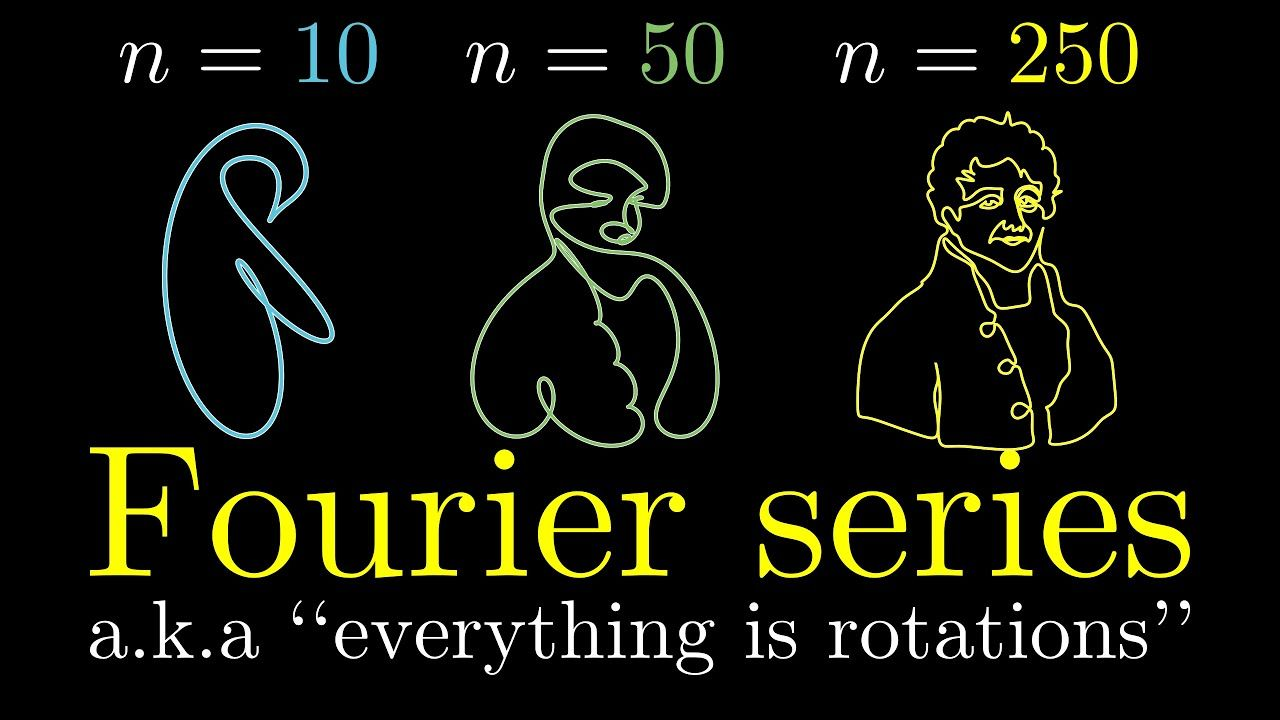
\includegraphics[width=0.8\paperwidth]{Res/img/fourier}
        };
    \end{frame}
    \begin{frame}{Linearna preslikavanja}
        Preslikavanje $f : \mathbb V \to \mathbb W$ je linearno ako važi:
        $$f(\alpha \vec x + \beta \vec y) = \alpha f(\vec x) + \beta f(\vec y)$$
        Tada je:
        $$f(\vec 0_{\mathbb V}) = \vec 0_{\mathbb W}$$
        Prostor svih linearnih preslikavanja $f : \mathbb V \to \mathbb W$ je vektorski
        prostor dimenzije $dim \mathbb V \cdot dim \mathbb W$
    \end{frame}
    \begin{frame}{Magični kvadrati}
        %\pause
        Sabiranje, množenje skalarom?
    \end{frame}
    \begin{frame}{Fibonačijevi nizovi}
        Koliko dimenzionalan je ovaj prostor?
    \end{frame}
    \begin{frame}{Igrice}
        Rotacije i izduživanja su linearne transformacije.
        Translacije 3D prostora su linearne transformacije 4D prostora.
        Projekcije 3D prostora na 2D ekran su linearne transformacije.
    \end{frame}
    \begin{frame}{Svadba}
        Mnogo ljudi došlo je na svadbu, zapravo ispostavilo se da su došli svi,
        odnosno na kraju nije više bilo mesta za sedenje. Međutim, niko nije bio obavešten o
        rasporedu sedenja. Koja je verovatnoća da niko nije seo na predviđeno mesto?
        (rešenje $e^{-1}$)
    \end{frame}
    \begin{frame}
        Hvala na pažnji!
    \end{frame}
    %\begin{frame}{Baza}
    \tiny
    \begin{align*}
        \begin{pmatrix}
            1&1&1&1\\
            1&1&1&1\\
            1&1&1&1\\
            1&1&1&1
        \end{pmatrix} &
        \begin{pmatrix}
            1&0&0&-1\\
            0&-1&1&0\\
            0&1&-1&0\\
            -1&0&0&1
        \end{pmatrix} &
        \begin{pmatrix}
            1&-1&0&0\\
            -1&1&0&0\\
            0&0&-1&1\\
            0&0&1&-1
        \end{pmatrix} &
        \begin{pmatrix}
            0&0&0&0\\
            1&0&0&-1\\
            -1&0&0&1\\
            0&0&0&0
        \end{pmatrix} \\
        \begin{pmatrix}
            1&0&-1&0\\
            0&-1&0&1\\
            -1&0&1&0\\
            0&1&0&-1
        \end{pmatrix} &
        \begin{pmatrix}
            0&0&-1&1\\
            0&0&1&-1\\
            1&-1&0&0\\
            -1&1&0&0
        \end{pmatrix} &
        \begin{pmatrix}
            0&-1&0&1\\
            1&0&-1&0\\
            0&1&0&-1\\
            -1&0&1&0
        \end{pmatrix} &
        \begin{pmatrix}
            0&1&-1&0\\
            0&0&0&0\\
            0&0&0&0\\
            0&-1&1&0
        \end{pmatrix}
    \end{align*}
\end{frame}

\end{document}
